\documentclass[12pt]{article}\usepackage[]{graphicx}\usepackage[]{color}
%% maxwidth is the original width if it is less than linewidth
%% otherwise use linewidth (to make sure the graphics do not exceed the margin)
\makeatletter
\def\maxwidth{ %
  \ifdim\Gin@nat@width>\linewidth
    \linewidth
  \else
    \Gin@nat@width
  \fi
}
\makeatother

\definecolor{fgcolor}{rgb}{0.345, 0.345, 0.345}
\newcommand{\hlnum}[1]{\textcolor[rgb]{0.686,0.059,0.569}{#1}}%
\newcommand{\hlstr}[1]{\textcolor[rgb]{0.192,0.494,0.8}{#1}}%
\newcommand{\hlcom}[1]{\textcolor[rgb]{0.678,0.584,0.686}{\textit{#1}}}%
\newcommand{\hlopt}[1]{\textcolor[rgb]{0,0,0}{#1}}%
\newcommand{\hlstd}[1]{\textcolor[rgb]{0.345,0.345,0.345}{#1}}%
\newcommand{\hlkwa}[1]{\textcolor[rgb]{0.161,0.373,0.58}{\textbf{#1}}}%
\newcommand{\hlkwb}[1]{\textcolor[rgb]{0.69,0.353,0.396}{#1}}%
\newcommand{\hlkwc}[1]{\textcolor[rgb]{0.333,0.667,0.333}{#1}}%
\newcommand{\hlkwd}[1]{\textcolor[rgb]{0.737,0.353,0.396}{\textbf{#1}}}%
\let\hlipl\hlkwb

\usepackage{framed}
\makeatletter
\newenvironment{kframe}{%
 \def\at@end@of@kframe{}%
 \ifinner\ifhmode%
  \def\at@end@of@kframe{\end{minipage}}%
  \begin{minipage}{\columnwidth}%
 \fi\fi%
 \def\FrameCommand##1{\hskip\@totalleftmargin \hskip-\fboxsep
 \colorbox{shadecolor}{##1}\hskip-\fboxsep
     % There is no \\@totalrightmargin, so:
     \hskip-\linewidth \hskip-\@totalleftmargin \hskip\columnwidth}%
 \MakeFramed {\advance\hsize-\width
   \@totalleftmargin\z@ \linewidth\hsize
   \@setminipage}}%
 {\par\unskip\endMakeFramed%
 \at@end@of@kframe}
\makeatother

\definecolor{shadecolor}{rgb}{.97, .97, .97}
\definecolor{messagecolor}{rgb}{0, 0, 0}
\definecolor{warningcolor}{rgb}{1, 0, 1}
\definecolor{errorcolor}{rgb}{1, 0, 0}
\newenvironment{knitrout}{}{} % an empty environment to be redefined in TeX

\usepackage{alltt}
\usepackage{latexsym}
\usepackage{fullpage}
\usepackage{graphicx}
\usepackage{endnotes}
\usepackage{epsfig}
\usepackage{setspace}
\usepackage{amsfonts}
\usepackage{caption}
\usepackage{threeparttable}
\usepackage[abbr]{harvard}
\usepackage{multirow}
\usepackage{longtable}
%\usepackage{times}
\usepackage{lscape}
\usepackage{float}
\usepackage{subfigure}
%\doublespacing
\IfFileExists{upquote.sty}{\usepackage{upquote}}{}
\begin{document}




\title{\textbf{Economic Growth,Performance Evaluation and Political Support in China: \large a test for modernization theory and `economic voting' theory}}
%\date{}
\bigskip
\onehalfspacing\author{
	Hao Wang \\ Department of Political Science\\Arizona State University\\haowang@asu.edu
	}
\maketitle \thispagestyle{empty}




\noindent \textbf{Keywords:} {Political Support, Economic Growth, Government Performance, China}

\bigskip

\noindent \textbf{Abstract:} {This manuscript tests two competing hypotheses of economic growth, performance evaluation and political support. According to the economic explanation of modernization theory, rapid economic growth fosters income inequality, and the poor will then demand political reform and redistribution of wealth. On the other hand, the cultural approach of modernization argues that socio-economic development changes value systems and people's ability to think critically. As a result, those people with higher levels of cognitive ability and political awareness will favor democracy in a authoritarian context. Meanwhile, Economic Voting literature argue that people value government's socio-economic performance, consequently they will support/oppose the incumbent government based on their evaluation. This study uses a general opinion survey in China to test these two competing hypotheses. My results show that cultural modernization mechanism is robust in all models}
\newpage

\doublespacing
\section{Introduction}
Since the Reform and Opening policy in 1978, China has undergone remarkably changes in economy, social structures and political structures. According to World Bank, China's GDP per capita increases from 154.97 USD in 1978 to 6807.43 USD in 2013, and World Bank has classified China as a `middle income' country. Dramatical changes in economic development secures Chinese Communist Party's (CCP) dominance in the post-Mao era (Holbig and Gilley 2010), many Chinese citizens express `special gratitude' to CCP for the remarkable increase of economy as well as their living standards. On the other hand, CCP justifies the authoritarian rule as `the only possible and correct' for Chinese people's sake, `Western Democracies are not suitable in China' (Yang and Chen 2013, Pei 2012).

Stable authoritarian ruling accompanied by rapid economic growth makes China a unique case in comparative politics. On one hand, economic development have dramatically shifted people's lifestyles: ordinary citizens can now afford modern appliances such as TV sets, computers, washing machines, automobiles etc., and many Chinese families can even send their children abroad for better education. Many scholars thus conclude that Chinese people are in favor of the strong nondemocratic governance because of rapid economic growth (Chen and Dickson 2008). On the other hand, economic growth does not unilaterally increase political support. Huntington (2008) made the famous argument that rapid economic growth often comes with dramatical changes of society, which brings about regime instability. With respect to the China case, economic growth brings about noticeable gaps between the rich and poor, government officials and the common citizens. Many Chinese citizens express their dissatisfaction of inequality, limited degrees of political rights and freedom of speech online (King 2013, Mackinoon 2011, Pan and Xu 2015). Protests on land reform and housing are not unusual titles in Chinese media (Li 2008, Kennedy 2008).

According to Modernization theory (Lipset 1959, 1993), economic growth will foster urbanization, industrialization, increasing levels of education and income, and as a result it will increase political participation and demand for democracy. Although the mechanism is challenged by Przeworski and Limongi (1997), still there is a general pattern between economic modernization and democracy. Since economic development not only changed Chinese citizen's physical well-beings but also cognitive ideas, it is worthwhile to test the relation between economic development and political attitudes towards a nondemocratic government (Zhai 2015).

On the other hand, retrospective evaluation theory holds that citizens value the economic performance of the government and vote accordingly (Lewis-Beck and Stegmaier 2000).  Although previous economic voting studies are based on democratic elections, there is no significant reason that citizens living in authoritarian countries would NOT value government performance. In fact, Lewis-beck et al. (2014) show that the vote-popularity function can be applied to nondemocratic settings like China. Therefore, instead of the negative relationship between economic development and demand for democracy; retrospective evaluation theory holds that good government performance will yield solid political support.

This project differs from the previous public opinion studies in that I incorporate provincial economic growth data into individual level surveys. Because there are significant variations of economic growth rates in different provinces, this allows me to test the two competing hypotheses simultaneously. Overall, this manuscript is trying to disentangle the relation between economic development and political attitudes in a nondemocratic environment. 


 




 
\nocite{HolbigGilley2010,YangChen2013,ChenDickson2008,Zhai2015,Lipset1993,Lipset1959,Lewis-Beck2000,Pan2015,Wallace2016}
\nocite{WorldBank1,WorldBank2,Kennedy2010,Lewis-Becketal2014,Truex2014,Li2008,Przeworski1997,Tsai2010,Meng2014,King2013,Huta2014}
\nocite{Rabe-Heskethetal2005,Rabe-Heskethetal2004,Pei2012,Mackinnon2011,Lorentzen2014,Huntington2008,Wintrobe1998,Boix2003a}

\section{Theory and Hypothesis}
\subsection{Modernization Theory}
Modernization theory holds that social-economic development includes a multi-stage process towards democracy. Accordingly, economic development will bring about higher levels of literacy, education, higher income and better living standards. It is argued that when people are economically better off, they will engage in many political activities and struggle for more political rights. This general pattern received some weak empirical support (such as Boix and Stokes 2003), but it has also been criticized for its unclear causal mechanism. Later Scholars refine modernization theory and propose two general causal mechanisms linking modernization and democratization together: through inequality and redistribution of wealth and through the transition of culture and values.


Economic explanations of modernization theory hold that inequality plays the pivotal role in triggering demand for redistribution (Acemoglu and Robinson 2005, Boix 2003), and consequently high levels of inequality will increase citizens' dissatisfaction on government and increase demand for political reform. According to Kuznets (1955), rapid economic growth
often comes with increasing gap of income inequality. And as a result of enlarging income inequality, people will demand political reform and redistribution. Therefore, we have:

\begin{quotation}
	Hypothesis 1 (Inequality): Rapid economic growth increases income gap, and consequently triggers people's demand for political democracy.
\end{quotation}

Cultural explanations of modernization theory focus on the changes in the social and cultural realms. It argues that modernization process enhances people's cognitive ability and critical thinking. Besides, the dramatic social-economic changes may influence previous value systems as well (Welzel et al. 2003). This explanation received support in political behavior and political psychology studies (e.g. Geddes and Zaller 1989, Zaller 1992, Truex 2014). With respect to the China case, Scholars also found empirical support for the Changing pattern of Chinese value system and ideology (Pan and Xu 2015, Yang and Tang 2010, Zhong and Chen 2013). Since authoritarian rules highlights obedience and respect to authority, it is inherently incompatible with critical thinking and self-expression values. A natural consequence is that people who think critically tend to be dissatisfied with authoritarian ruling:

\begin{quotation}
	Hypothesis 2 (Critical Thinking): Modernization process increases citizens' ability of thinking critically (about politics), consequently they will demand more political rights and higher levels of liberty.
\end{quotation}
\nocite{Kuznets1955,Welzeletal2003}
\nocite{Acemoglu2005,Boix2003}


\subsection{`Economic Voting' Theory}
Unlike modernization theory which depicts the path to democracy as a unidimensional route, `economic voting' literatures model political support as a function of government performance, especially on economic and social issues (Lewis-Beck and Stegmaier 2000). Although citizens in a authoritarian country do not vote the way in democracies, they can express their opinions in informal ways. For instance, in a village-level field Lily Tsai identifies that `accountability' exists in rural China (Tsai 2007). Therefore, a natural hypothesis is that people who highly evaluate government performance in socio-economic issues tend to support the incumbent elites. Unfortunately, the data structure I have does not contain important questions on socio-tropic evaluation; nevertheless, the CGSS 2003 survey includes related questions on `pocket book' voting, respondents were asked to compare their income and living condition to 3 years ago/5 years ago and 10 years ago, as well as prospective evaluation (compare with what it may be 3 years/5 year/10 years later). Consequently we have the following two hypotheses:

\begin{quotation}
	Hypothesis 3 (Retrospective Evaluation): Citizens whose economic condition increased/decreased over the past years tend to support incumbent governance/political reforms
\end{quotation}

\begin{quotation}
	Hypothesis 4 (Prospective Evaluation): Citizens who expect their economic condition will increase/decrease in the future years tend to support incumbent governance/political reforms
\end{quotation}

Overall, I highlight four possible mechanisms linking economic development with political support.
%Modernization hypothesis is developed exclusively in explaining regime transitions. On the other hand, `Economic Voting' literature comes from experiences in Western democracies.
 According to Przeworski and Limongi (1997), China should be in transition to democracy as it has passed the `transition bar' of \$4000. However, China seems to be a stable autocracy now and since CCP is in control of the military, a coup is unlikely. On the other hand, one might doubt the applicability of `Economic Voting' theory in a nondemocratic context: can authoritarian leaders generate political support by rapid economic development? This study provides a test for both theories based on survey data in China as well as provincial level economic growth indicators.
  







\nocite{Tsai2007a}
  






\section{Data and Method}
\subsection{Data Description}
Data in this study comes from two sources: provincial level economic growth data is collected from China Compendium of Statistics (1950-2009), Figure \ref{growth} shows the average provincial level growth rate from year 2001 to year 2005. As shown in the map, there are noticeable provincial level variations in economic growth. In general, coastal provinces tend to grow faster than inner provinces. Inner Mongolia and Shanxi Province also have a high GDP growth rate, however these provinces heavily rely on their natural resources.


\begin{figure}[H]
	\centering
	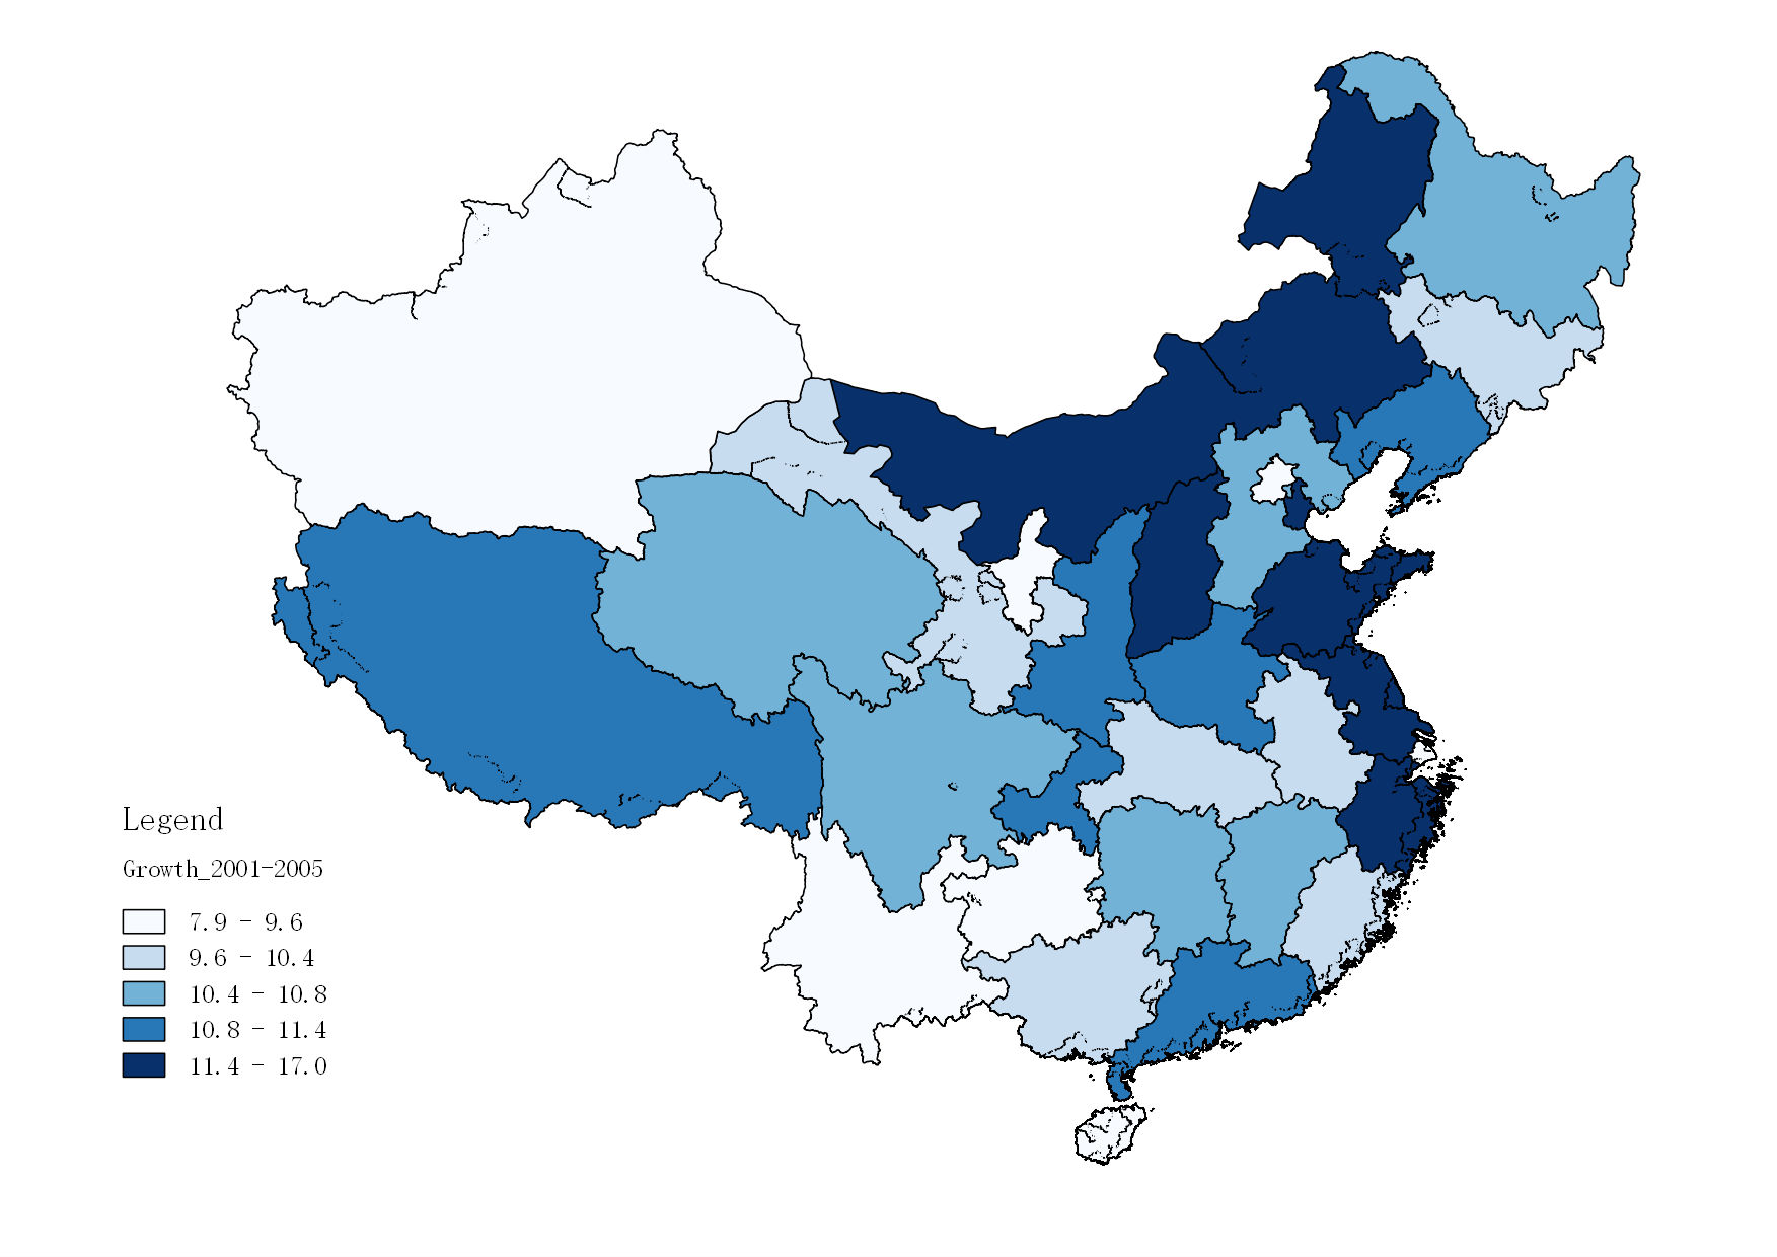
\includegraphics[width=1\textwidth]{growth}
	\caption{\label{growth} Provincial Level Average GDP Growth Rate, 2001-2005}
\end{figure}	


Individual level data is from the 2006 China General Social Survey (CGSS). CGSS is a annual/biannual survey of China's urban and rural households and it started at 2003. Comparing with other surveys such as China Value 
and Ethnic Survey (featured in Yang and Tang 2010) and World Value Survey, CGSS comes with a more representative sample and much larger observations. The survey was administered by Renmin University and other regional institutions in China. In 2006, the survey was conducted between September and November, 10151 households in 28 provinces (out of 31) were interviewed. Although this survey did not focus on citizens' political opinion, it nevertheless provide questions directly and indirectly reflecting people's political preferences (Jiang and Yang 2015). Response rate in the 2006 survey was about 51.10\% and the missing value rate was about 3.41$\%$.

\subsection{Dependent Variable}
I use two different dependent variables in this manuscript to measure trust in government and demand for democracy. CGSS 2006 asks many related questions on politics, governance and political reform. With respect to political trust, CGSS asks respondents to rate the credibility of government official announcements based on the following question setting:
\begin{quotation}
	To what degree do you trust government reports/announcements on: housing; stock market; employment situation for college graduates; corruption; income inequality; domestic security; deaths in mining industry; deaths in earthquake
\end{quotation} 
Ratings range from ``Not trust at all" to ``completely trust''. I reversed the coding scale to make it positively related to trust in government. 
Since this question ask people's attitude towards government, one concern is that people may perform self-censorship and hide their responses (Lozenren 2014, Jiang and Yang 2015). While there is no sufficient mechanism to tease out the `inflated' support for government, the unresponsive rates of these questions are as low as 1\%. Self-censorship and social desirability bias is a real challenge in conducting opinion research in nondemocracies. Scholars point out that citizens tend to fake their preferences to escape from potential punishment (Wintrobe 1998, Li 2008). In an extreme condition when everyone hides his true ideas, we may observe uniformly high levels of political trust and political support. Fortunately the responses of trust question have a good amount of variation. Since we assume the survey data on political trust will be inflated, statistically it will show less variations of dependent variable and make it less likely to display statistically significant patterns. In other words, if we can detect significant results when dependent variable is inflated, our results should be robust under `true' conditions. The raw distributions of responses on government trust are shown below:

According to Figure \ref{Trust}, it shows that about 15\% to 20\% citizens do not trust government reports. Considering the mechanism of self-censorship, the actual proportion of people who do not trust government may be larger.

The second dependent variable that I use is political support for the CCP governance. I model demand for democracy based on the following question in CGSS:
\begin{quotation}
	Do you agree or disagree with the following argument: as long as economy is good, there is no need for political reform and democracy
\end{quotation}

The distribution of the reponses is shown in Figure \ref{democracy}. Unlike the Trust in Government question, Demand for Democracy question has a higher nonresponse rate. It is somewhat expected because political reform or democracy is sensitive topic. However, unlike the trust in Government question in which the majority of respondents support the Government, in Democracy question nearly half of the respondents require political reform and democracy.

\begin{figure}[H]
	\centering
	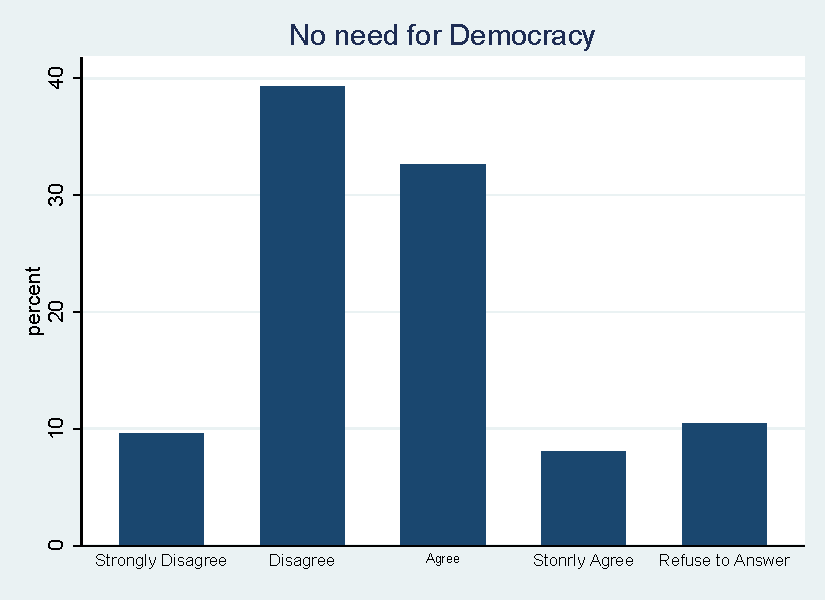
\includegraphics[width=90mm]{Democracy}
	\caption{\label{democracy} No need for Democracy when economy is good}
\end{figure}	




 \begin{figure}[H]
 	\centering
 	\subfigure[Housing]{\label{fig:a}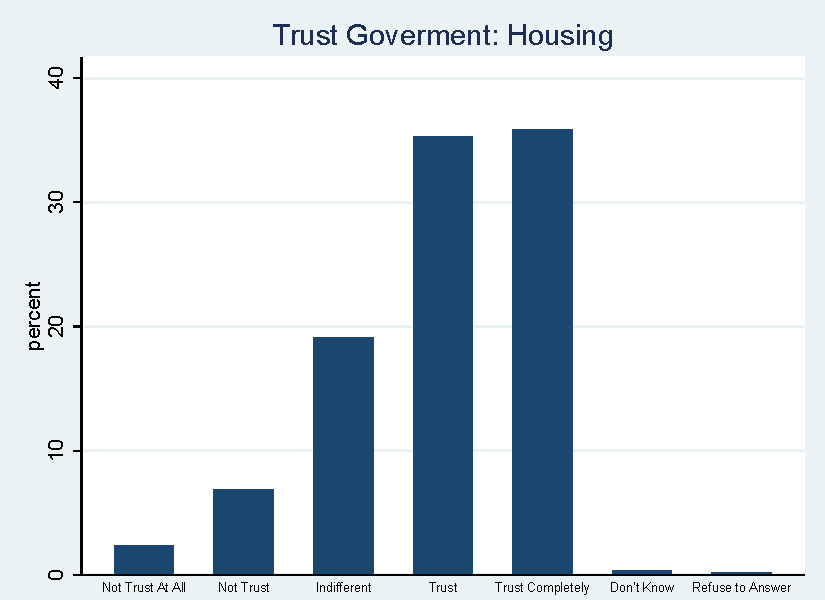
\includegraphics[width=80mm]{TrustGov1}}
 	\subfigure[Stock Market]{\label{fig:b}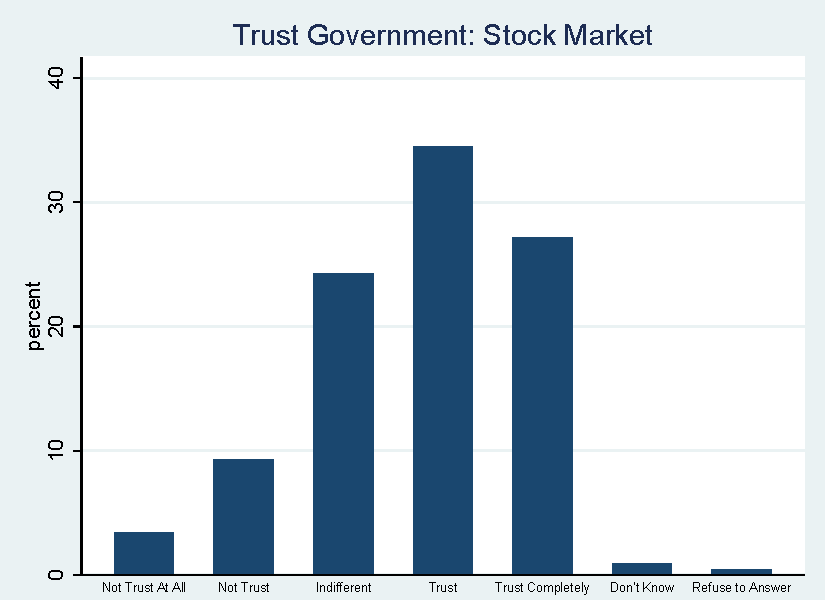
\includegraphics[width=80mm]{TrustGov2}}
 	\subfigure[Corruption]{\label{fig:c}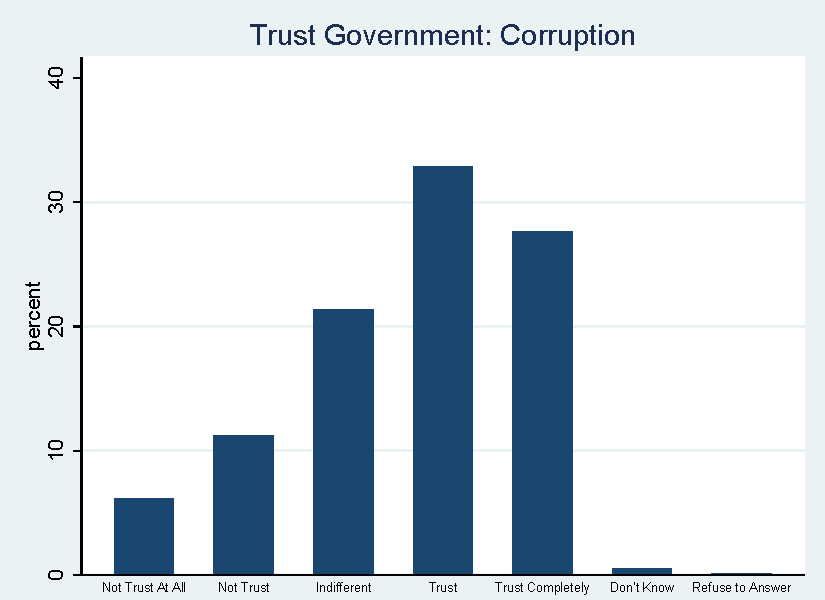
\includegraphics[width=80mm]{TrustGov3}}
 	\subfigure[Inequality]{\label{fig:ba}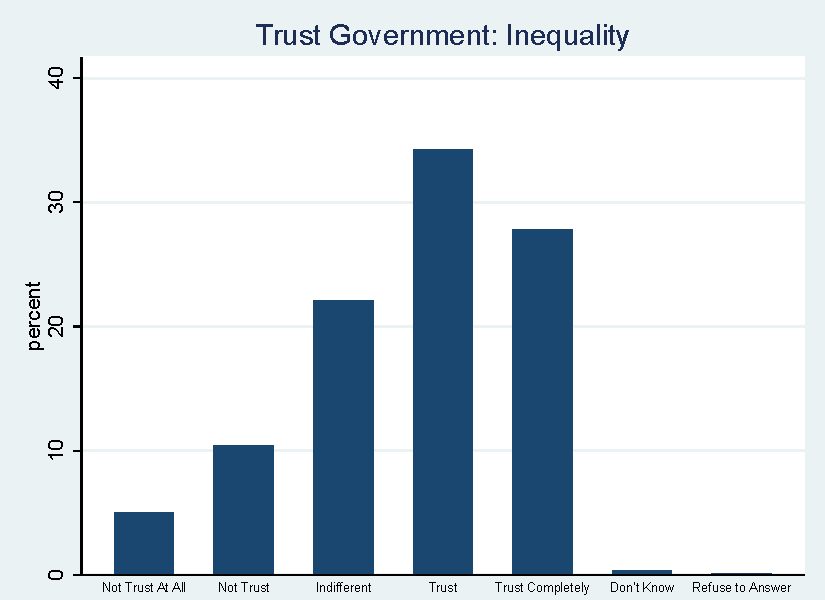
\includegraphics[width=80mm]{TrustGov4}}
 	\subfigure[Employment]{\label{fig:bb}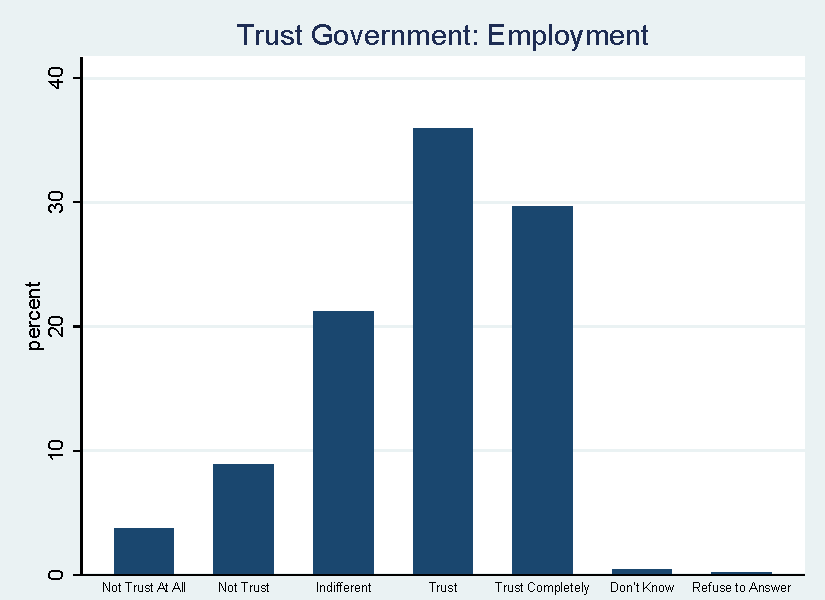
\includegraphics[width=80mm]{TrustGov5}}
 	\subfigure[Security]{\label{fig:bc}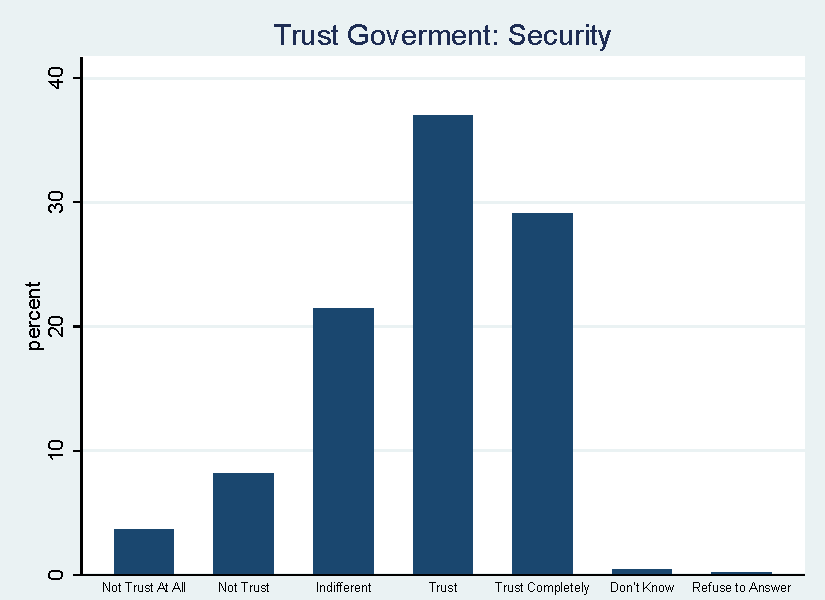
\includegraphics[width=80mm]{TrustGov6}}
 	%\caption{Histograms and Boxplots for Model 1}
 \end{figure}


\begin{figure}
	\centering
		\subfigure[Mining Accident]{\label{fig:bd}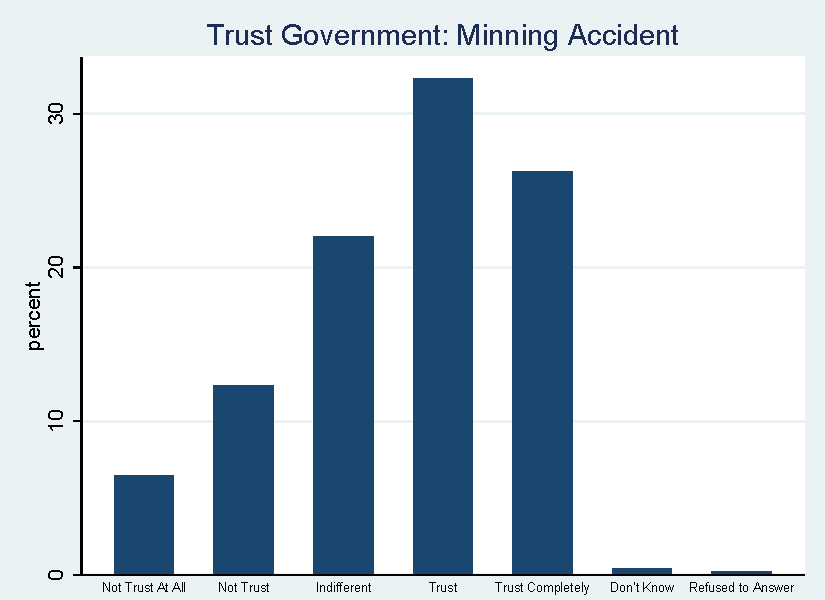
\includegraphics[width=80mm]{TrustGov7}}
		\subfigure[Earthquake]{\label{fig:be}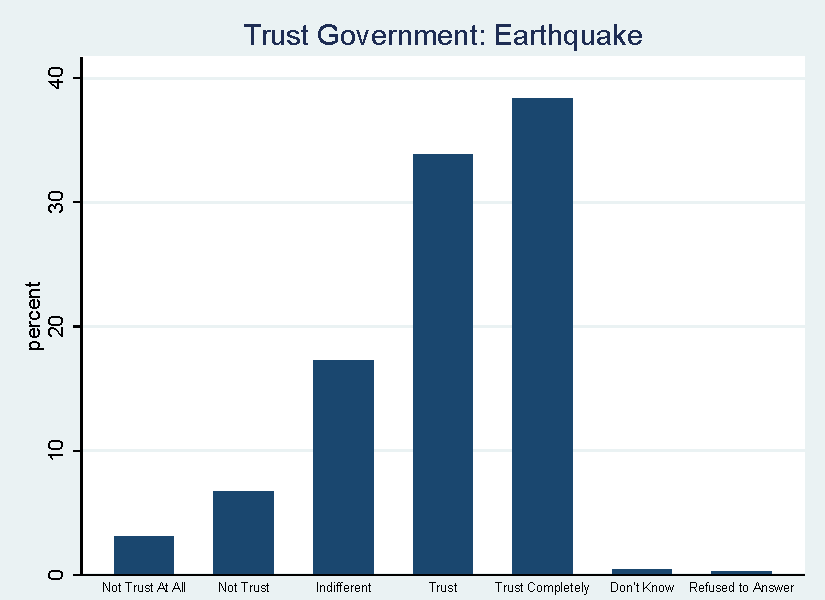
\includegraphics[width=80mm]{TrustGov8}}
		\caption{\label{Trust} Distribution of Trust in Government}
\end{figure}

\subsection{Independent Variable}
The main independent variables in this study is economic growth, critical thinking ability and economic evaluation. Economic growth is models as provincial-level average GDP growth rate before 2006 (which is the survey year), I calculated 3-year average, 5-year average and 10-year average respectively. This is the level-2 data in my analysis, and based on modernization theory, we should have the following two paths:
\begin{itemize}
\item	Path 1: Economic growth $\Rightarrow$ Increased Income Inequality $\Rightarrow$ less support for the CCP government and demand for democracy 
\item	Path 2: Economic growth $\Rightarrow$ Ability to Think Critically $\Rightarrow$ less support for the CCP government and demand for democracy 
\end{itemize}

\noindent Income inequality is based on the following question:
\begin{quotation}
	What do you think of the tension between the rich and the poor: very serious; serious; not that much; no conflict at all.
\end{quotation}
The basic distribution is shown in Figure \ref{rich}
\begin{figure}[H]
	\centering
	\includegraphics[width=90mm]{rich_poor}
	\caption{\label{rich} Tension Between thr Rich and Poor}
\end{figure}

Critical Thinking is based on the following 3 questions, distributions are shown in Figure \ref{Critical}.

\begin{itemize}
	\item It is always good to follow the government decisions (range from strongly agree to strongly disagree)
	\item Law should be based on government decisions (range from strongly agree to strongly disagree)
	\item Politics is too complicated that I cannot understand (range from strongly agree to strongly disagree)
\end{itemize}


\begin{figure}
	\centering
	\subfigure[Following Government]{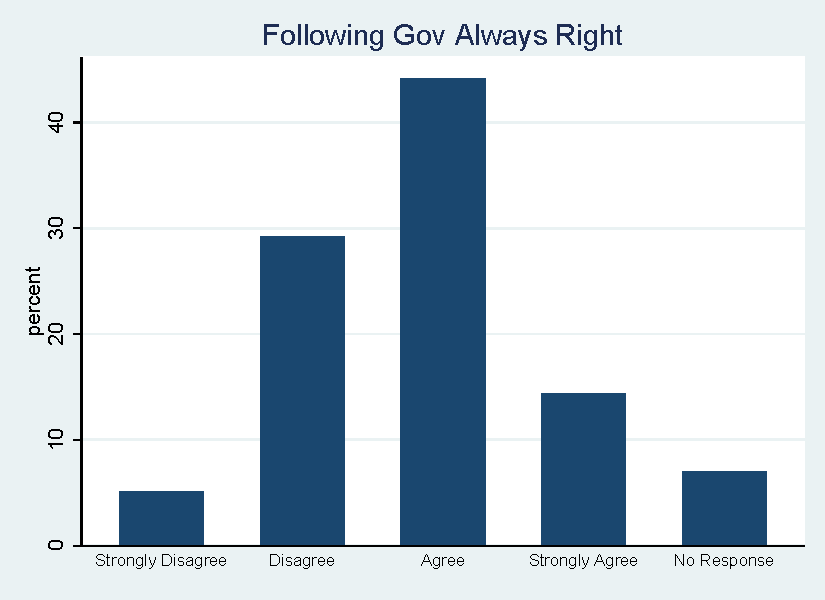
\includegraphics[width=80mm]{cri_gov}}
	\subfigure[Government Over Law]{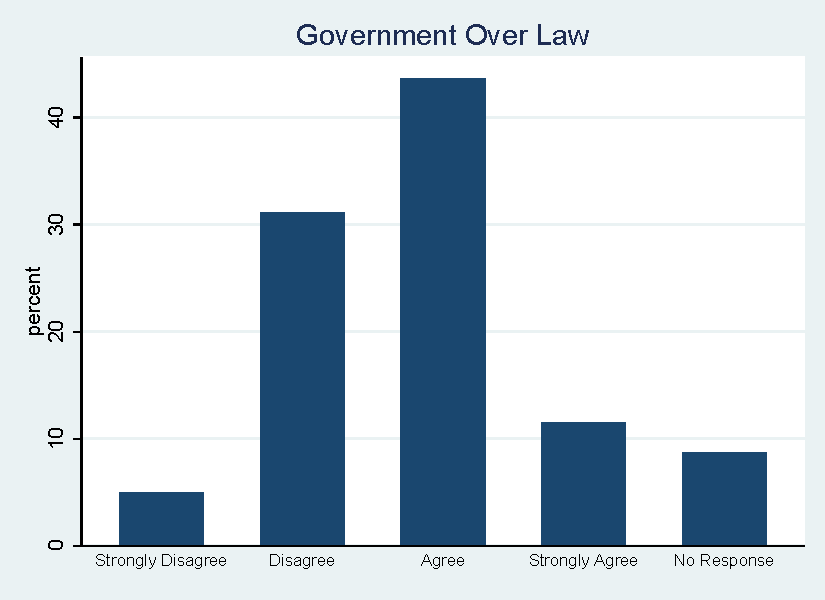
\includegraphics[width=80mm]{law_gov}}
	\subfigure[Politics Complicated]{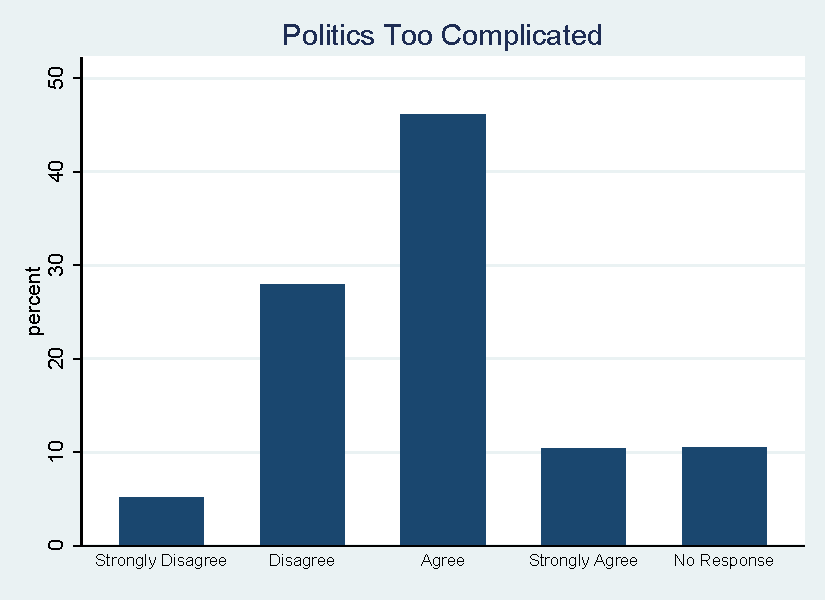
\includegraphics[width=80mm]{poli_interest}}
	\caption{\label{Critical} Distribution of Critical Thinking Components}
\end{figure}


	
I model economic evaluation on retrospective evaluation and prospective evaluation. Retrospective evaluation is based on the following questions from CGSS 2006:
\begin{quotation}
	Compare to 3 years ago, your income/asset/position/working condition/social class has: increased/no changes/decreased
\end{quotation}
Prospective self-evaluation is based on similar questions but respondents were asked about their expectations in the future.
\begin{quotation}
	What is your expectation of your income/asset/position/working condition/social class after 3 years: increase/no changes/decrease
\end{quotation}
According to retrospective evaluation theory, we will have the following patterns:

\begin{itemize}
	\item Positive retrospective evaluation is related to positive attitude towards government and less demand for democracy.
	\item Negative retrospective evaluation is related to negative attitude towards government and more demand for democracy.
	\item Positive Prospective evaluation is related to positive attitude towards government and less demand for democracy.
	\item Negative Prospective evaluation is related to negative attitude towards government and more demand for democracy.
\end{itemize}

I also include other demographic variables like CCP party membership, gender, age, household income and education.







\subsection{Method}
%Since I include level 1 individual-level survey data and level 2 provincial level GDP growth data. I use multilevel modeling in the analysis part. I use both multi-level linear model and multi-level structural equation model (SEM) in testing the previous hypotheses (Huta 2014). SEM has an edge over linear model here because both trust in government and self-evaluation are measured in multiple attributes (Rabe-Hesketh et al. 2004, 2005). Besides, path analysis is feasible in SEM, which can test modernization theory in one single model. On the other hand, linear model coefficients are easier to interpret, therefore I provide two models here\footnote{I'm still figuring out the convergence issue of gsem, will add results from gsem later}. 

%In HLM (Hierarchical Linear Model) trust in government and self-evaluation are modeled by aggregated mean values. And in SEM, Trust in government and Self-evaluation is modeled as latent variables. 






\nocite{YangTang2010,JiangYang2015}


\section{Result}
Results from HLM is shown in Table \ref{modernization} and Table \ref{evaluation}.
Model (1) to (3) in Table \ref{modernization} show the regression results when dependent variable is Trust in Government. Model (4) to (6) show regression results when dependent variable is Demand for Democracy.
From Table \ref{modernization}, we found three our of the four indicators of modernization mechanism are statistically significant. Inequality is negatively related to the trust in government support for democracy. Critical Thinking variables (critical gov, gov over law and politics complicated) show negative signs in the trust of Government, however they display positive attitudes towards democracy. Economic growth rates do not have an impact on trust in government nor demand for democracy. People who live in urban districts show less confidence on government credibility and hider demands for democracy. Surprisingly education does not have an impact on trust in government nor support for democracy. There are moderate effects (though statistically significant) of Age in support democracy. The negative signs show that older people tend to support the current regime more.
Foreign language speaking ability shows somewhat negative relation to Trust in Government, although it is not significant in Model (2). The last control variable measures CCP party membership, the results are unexpected: party members tend to support political reforms and democracy. 



%\footnote{Note: Critical Gov: It is always good to support government; Gov over Law: Law should be based on government decisions; Politics Complicated: Politics too complicated for me to understand}+
% Table generated by Excel2LaTeX from sheet 'Sheet1'
\begin{table}[htbp]
	\centering
	\caption{\label{modernization} Testing Modernization Hypothesis on Multilevel Linear Model}
	\begin{tabular}{lrrrrrr}
	
		\hline
		& \multicolumn{1}{c}{(1)} & \multicolumn{1}{c}{(2)} & \multicolumn{1}{c}{(3)} & \multicolumn{1}{c}{(4)} & \multicolumn{1}{c}{(5)} & \multicolumn{1}{c}{(6)} \\
		Var   & \multicolumn{1}{c}{TrustGov} & \multicolumn{1}{c}{TrustGov} & \multicolumn{1}{c}{TrustGov} & \multicolumn{1}{c}{Democracy} & \multicolumn{1}{c}{Democracy} & \multicolumn{1}{c}{Democracy} \\
		& \multicolumn{1}{c}{} & \multicolumn{1}{c}{} & \multicolumn{1}{c}{} & \multicolumn{1}{c}{} & \multicolumn{1}{c}{} & \multicolumn{1}{c}{} \\
		\hline
	 Inequality & -0.0578*** & -0.0690*** &       & -0.0247** & -0.0286*** &  \\
	 & (0.00967) & (0.0105) &       & (0.00977) & (0.00968) &  \\
	 Critical\_Gov &       & -0.167*** & -0.170*** &       & 0.0856*** & 0.0816*** \\
	 &       & (0.0128) & (0.0127) &       & (0.0117) & (0.0116) \\
	 Gov over Law &       & -0.0553*** & -0.0561*** &       & 0.212*** & 0.213*** \\
	 &       & (0.0132) & (0.0131) &       & (0.0120) & (0.0120) \\
	 Politics Complicated &       & 0.0111 & 0.0106 &       & 0.267*** & 0.266*** \\
	 &       & (0.0126) & (0.0125) &       & (0.0115) & (0.0115) \\
	 Ave 3-year Growth & 0.0561 & 0.101 & 0.0733 & -0.0148 & -0.0341 & -0.0397 \\
	 & (0.0813) & (0.0844) & (0.0850) & (0.0732) & (0.0591) & (0.0592) \\
	 Ave 5-year Growth & 0.0119 & -0.135 & -0.123 & -0.162 & -0.0282 & -0.0222 \\
	 & (0.152) & (0.155) & (0.157) & (0.135) & (0.107) & (0.108) \\
	 Ave 5-year Growth & -0.0238 & 0.0699 & 0.0722 & 0.121 & 0.0314 & 0.0299 \\
	 & (0.0970) & (0.0997) & (0.101) & (0.0867) & (0.0691) & (0.0696) \\
	 Urban & -0.0696*** & -0.0453** & -0.0572** & 0.121*** & 0.0776*** & 0.0725*** \\
	 & (0.0208) & (0.0225) & (0.0224) & (0.0208) & (0.0206) & (0.0204) \\
	 Gender: Male & -0.0246 & -0.0284 & -0.0241 & 0.0582*** & 0.0247 & 0.0228 \\
	 & (0.0177) & (0.0191) & (0.0190) & (0.0177) & (0.0175) & (0.0174) \\
	 Education & -0.00915 & -0.00457 & -0.00312 & 0.00365 & -0.00943 & -0.00918 \\
	 & (0.0111) & (0.0121) & (0.0120) & (0.0112) & (0.0110) & (0.0109) \\
	 Age   & -0.000572 & -0.000444 & -0.000654 & -0.00284*** & -0.00241*** & -0.00238*** \\
	 & (0.000774) & (0.000834) & (0.000829) & (0.000773) & (0.000765) & (0.000759) \\
	 Income & 5.49e-08 & 2.31e-08 & 4.38e-08 & 2.57e-08 & -6.18e-08 & -4.71e-08 \\
	 & (5.24e-08) & (6.80e-08) & (6.72e-08) & (5.00e-08) & (6.12e-08) & (6.04e-08) \\
	 Foreign Language & -0.0373*** & -0.0206 & -0.0253* & 0.00691 & -0.00881 & -0.00805 \\
	 & (0.0138) & (0.0147) & (0.0146) & (0.0135) & (0.0133) & (0.0133) \\
	 Party Membership & -0.00469 & -0.00512 & -0.00112 & 0.116*** & 0.0576* & 0.0669** \\
	 & (0.0320) & (0.0342) & (0.0339) & (0.0314) & (0.0311) & (0.0308) \\
	 Constant & 3.651*** & 4.119*** & 4.088*** & 3.088*** & 1.677*** & 1.619*** \\
	 & (0.339) & (0.358) & (0.361) & (0.309) & (0.258) & (0.257) \\
	 &       &       &       &       &       &  \\
	 Observations & 8,914 & 7,452 & 7,605 & 8,112 & 7,188 & 7,325 \\
	 Number of groups & 28    & 28    & 28    & 28    & 28    & 28 \\ 
		\hline
		\multicolumn{7}{c}{Standard errors in parentheses} \\
		\multicolumn{7}{c}{*** p$<$0.01, ** p$<$0.05, * p$<$0.1} \\
	\end{tabular}\\
\end{table}%


Table \ref{evaluation} show the result of testing `Economic Voting' theory. Since this theory emphasizes self-evaluation of economic conditions rather than the objective economic growth, I exclude GDP growth rates in this test. Overall, we only find very weak support for self-evaluation theory. People who believe that their economic condition will become better tend to trust government more. However there is no statistically significant effect of retrospective evaluation and Trust in Government. On the other hand, modernization variables are very consistent with Table \ref{modernization}. People who highlight the issue of income inequality tend to trust government less, and show less support for democracy. However, for people who think critically, they tend to show less favorable attitudes towards government and more favorable to democracy.

% Table generated by Excel2LaTeX from sheet 'Sheet1'
\begin{table}[htbp]
	\centering
	\caption{\label{evaluation}Testing Economic Voting Models}
	\begin{tabular}{lcccccc}
		\hline
		& (1)    & (2)    & (3)   & (4)  & (5)  & (6) \\
	
		VAR & TrustGov & TrustGov & TrustGov & Democracy & Democracy &Democracy \\
		&       &       &       &       &       &  \\
		\hline
		Prospective &       & 0.0892*** & 0.0917*** &       & 0.0159 & 0.00748 \\
		&       & (0.0192) & (0.0241) &       & (0.0193) & (0.0222) \\
		Retrospective & 0.0236 &       & -0.0226 & 0.0138 &       & -0.00125 \\
		& (0.0190) &       & (0.0230) & (0.0189) &       & (0.0212) \\
		Inequality &       &       & -0.0605*** &       &       & -0.0251** \\
		&       &       & (0.0106) &       &       & (0.00985) \\
		Cri Gov &       &       & -0.163*** &       &       & 0.0911*** \\
		&       &       & (0.0129) &       &       & (0.0119) \\
		Gov Over Law &       &       & -0.0592*** &       &       & 0.202*** \\
		&       &       & (0.0134) &       &       & (0.0123) \\
		Politics Complicated &       &       & 0.00628 &       &       & 0.263*** \\
		&       &       & (0.0127) &       &       & (0.0117) \\
		Urban & -0.0819*** & -0.0760*** & -0.0418* & 0.116*** & 0.115*** & 0.0780*** \\
		& (0.0209) & (0.0205) & (0.0229) & (0.0210) & (0.0207) & (0.0210) \\
		Gender & -0.0204 & -0.0224 & -0.0258 & 0.0600*** & 0.0581*** & 0.0264 \\
		& (0.0177) & (0.0175) & (0.0193) & (0.0177) & (0.0175) & (0.0177) \\
		Education & -0.0102 & -0.0113 & -0.00758 & 0.00735 & 0.00218 & -0.00630 \\
		& (0.0111) & (0.0110) & (0.0122) & (0.0112) & (0.0110) & (0.0112) \\
		Age   & -0.000427 & 0.000107 & 0.000464 & -0.00262*** & -0.00280*** & -0.00214*** \\
		& (0.000781) & (0.000784) & (0.000867) & (0.000780) & (0.000786) & (0.000798) \\
		Income & 6.84e-08 & 6.62e-08 & 2.22e-08 & 3.66e-08 & 3.23e-08 & -5.69e-08 \\
		& (5.20e-08) & (5.21e-08) & (6.78e-08) & (4.95e-08) & (4.96e-08) & (6.13e-08) \\
		Foreign Language & -0.0306** & -0.0446*** & -0.0155 & 0.00520 & 0.00573 & -0.00886 \\
		& (0.0142) & (0.0137) & (0.0153) & (0.0140) & (0.0135) & (0.0140) \\
		Party & -0.00867 & -0.00443 & -0.00627 & 0.118*** & 0.126*** & 0.0561* \\
		& (0.0318) & (0.0316) & (0.0343) & (0.0312) & (0.0310) & (0.0314) \\
		Constant & 3.848*** & 3.689*** & 4.284*** & 2.522*** & 2.538*** & 1.380*** \\
		& (0.0781) & (0.0819) & (0.105) & (0.0749) & (0.0798) & (0.0920) \\
		&       &       &       &       &       &  \\
		Observations & 8,920 & 9,197 & 7,264 & 8,067 & 8,296 & 7,002 \\
		Number of groups & 28    & 28    & 28    & 28    & 28    & 28 \\
		\hline
		\multicolumn{7}{c}{Standard errors in parentheses} \\
		\multicolumn{7}{c}{*** p$<$0.01, ** p$<$0.05, * p$<$0.1} \\

	\end{tabular}%
\end{table}%






\newpage

\section{Alternative Mechanism: an information model based on censorship}
Memory-based model argues that people's attitude is drawn from the most recent memory (Zaller 1992). Consequently one might need to think about the effect of media coverage in the authoritarian context (King et al. 2013, 2016; Mackinnon 2011). TV news reports by the central TV station speak in a favorable tone to the CCP governance. Similarly, government-owned newspaper like ``Poeple's Daily", which is the largest newspaper company in China, is known as standing in the same line with Chinese Communist Party \footnote{Internet usage may bring out another self-selection issue: people who are dissatisfied with the government-dominated media may turn to the Internet. Fortunately this is not a serious issue in CGSS 2006: most people (76\% of the total respondents) do not have access to the Internet}. Geddes and Zaller (1989) argue that media exposure has different impacts on people who think critically or not. For those who have higher levels of political awareness, they can resist the influence of the government dominated media. Therefore, we may expect a mediation effect through the ability of critical thinking:

\begin{itemize}
	\item Media exposure has less impact on government support among those who think critically about politics
	\item Media exposure increase government support among those who do not think critically about politics
\end{itemize}

To model the influence of media, I add media exposure (average frequency score of TV and Newspaper) and an Interaction term, Results are shown in the following table \ref{media}. According to the regression outputs, media exposure (newspaper) has no impact on democracy, but has some influence on political trust. However, it seems critical thinking  ability cannot resist media exposure since the interaction term is positive.


% Table generated by Excel2LaTeX from sheet 'Sheet1'
\begin{table}[htbp]
	\centering
	\caption{\label{media} Media Exposure and Political Attitudes : Potential Interaction}
	\begin{tabular}{lcccc}
		\hline
		& (1)   & (2)   & (3)   & (4) \\
		VAR   & TrustGov & TrustGov & Democracy & Democracy \\
		&       &       &       &  \\
		\hline
		Inequality & -0.0702*** & -0.0708*** & -0.0299*** & -0.0299*** \\
		& (0.0105) & (0.0105) & (0.00968) & (0.00968) \\
		Cri Gov & -0.166*** & -0.275*** & 0.0860*** & 0.105 \\
		& (0.0128) & (0.0990) & (0.0117) & (0.0901) \\
		TV    & -0.0188* & -0.0279 & -0.00704 & 0.00106 \\
		& (0.0107) & (0.0339) & (0.00993) & (0.0307) \\
		TV*Cri &       & 0.00447 &       & -0.00368 \\
		&       & (0.0146) &       & (0.0133) \\
		Newspaper & 0.0185*** & -0.0245** & 0.0166*** & 0.0137 \\
		& (0.00507) & (0.0121) & (0.00463) & (0.0111) \\
		Newspaper*Cri &       & 0.0192*** &       & 0.00131 \\
		&       & (0.00490) &       & (0.00448) \\
		Gov Over Law & -0.0563*** & -0.0559*** & 0.211*** & 0.211*** \\
		& (0.0132) & (0.0131) & (0.0120) & (0.0120) \\
		Politics Complicated & 0.00796 & 0.00800 & 0.264*** & 0.264*** \\
		& (0.0126) & (0.0126) & (0.0116) & (0.0116) \\
		Urban & -0.0778*** & -0.0785*** & 0.0494** & 0.0492** \\
		& (0.0242) & (0.0242) & (0.0221) & (0.0221) \\
		Gender & -0.0351* & -0.0347* & 0.0199 & 0.0199 \\
		& (0.0192) & (0.0191) & (0.0176) & (0.0176) \\
		Education & -0.0167 & -0.0172 & -0.0215* & -0.0216* \\
		& (0.0127) & (0.0127) & (0.0116) & (0.0116) \\
		Age   & -0.000407 & -0.000519 & -0.00241*** & -0.00241*** \\
		& (0.000834) & (0.000833) & (0.000764) & (0.000765) \\
		Income & 1.75e-08 & 1.47e-08 & -6.66e-08 & -6.66e-08 \\
		& (6.80e-08) & (6.79e-08) & (6.12e-08) & (6.12e-08) \\
		Foreign & -0.0251* & -0.0267* & -0.0119 & -0.0121 \\
		& (0.0147) & (0.0147) & (0.0134) & (0.0134) \\
		Party & -0.0134 & -0.0123 & 0.0498 & 0.0499 \\
		& (0.0343) & (0.0343) & (0.0312) & (0.0312) \\
		Constant & 4.628*** & 4.873*** & 1.462*** & 1.420*** \\
		& (0.108) & (0.241) & (0.0962) & (0.218) \\
		&       &       &       &  \\
		Observations & 7,452 & 7,452 & 7,188 & 7,188 \\
		Number of groups & 28    & 28    & 28    & 28 \\
		\hline
		\multicolumn{5}{c}{Standard errors in parentheses} \\
		\multicolumn{5}{c}{*** p$<$0.01, ** p$<$0.05, * p$<$0.1} \\
		
	\end{tabular}%
\end{table}%


\section{Discussion}
So far this manuscript analyzes two competing theories: modernization hypothesis and `Economic Voting' literatures (performance evaluation model). My results show that the two approaches of modernization theory predicts government trust and demand for democracy consistently. Inequality remains negatively correlated with government, which is as expected. However, inequality is negatively related to demand for democracy as well. This indicates that for those who emphasize the importance of inequality; their demand are still in economic domain and there is no `spillover' effect of linking Democracy to less inequality. This finding challenges the economic explanation of democratization and redistribution (e.g. Boix 2003). On the other hand, the cultural explanation of value shifts and ability of critical thinking goes consistently with the theoretical prediction. Future study on public opinion research in nondemocratic countries may keep a record of value change.

Another issue here is the possible self-censorship problem in surveys like CGSS. For instance, there are about 10\% nonresponse rates in the Critical Thinking questions. This is a much higher rate than the previous attribute questions. It is highly likely that respondents are hiding their true opinions. Jiang and Yang (2015) analyze the difference between `less sensitive' and `sensitive' questions to detect the problem of self-censorship. Alternatively, there're many experimental studies using list experiments (Meng et al. 2014) and Implicit Association Test. Combining survey researches and experiment studies together may provide us with a better understanding of public opinion in nondemocratic countries like China.




\nocite{GeddesZaller1989}




\newpage
\bibliography{D:/Dropbox/Bibliography-database/Haowang}
%\bibliography{~/Dropbox/Bibliography-database/Haowang}
%\bibliography{Haowang}
\bibliographystyle{apsr}





\end{document}
